%%%%%%%%%%%%%%%%%%%%%%%%%%%%%%%%%%%%%%%%%
% Thin Sectioned Essay
% LaTeX Template
% Version 1.0 (3/8/13)
%
% This template has been downloaded from:
% http://www.LaTeXTemplates.com
%
% Original Author:
% Nicolas Diaz (nsdiaz@uc.cl) with extensive modifications by:
% Vel (vel@latextemplates.com)
%
% License:
% CC BY-NC-SA 3.0 (http://creativecommons.org/licenses/by-nc-sa/3.0/)
%
%%%%%%%%%%%%%%%%%%%%%%%%%%%%%%%%%%%%%%%%%

%----------------------------------------------------------------------------------------
%	PACKAGES AND OTHER DOCUMENT CONFIGURATIONS
%----------------------------------------------------------------------------------------

\documentclass[a4paper, 10pt,twocolumn]{article} % Font size (can be 10pt, 11pt or 12pt) and paper size (remove a4paper for US letter paper)
\usepackage{geometry}
\geometry{left=1.3cm, right=1.3cm, top=1.3cm, bottom=1.3cm}
\usepackage{listings}   
\usepackage{amsmath}
\usepackage{wrapfig} % Allows in-line images
\usepackage{graphicx}
\usepackage{mathpazo} % Use the Palatino font
\usepackage[T1]{fontenc} % Required for accented characters
\usepackage{floatrow}
\usepackage{lmodern}
\usepackage{graphicx}
\usepackage{amsthm}
\usepackage{float}
\usepackage{ctable} 
\newtheorem*{theorem*}{Theorem}
\newtheorem*{corollary*}{Corollary}
\usepackage{lingmacros}
\usepackage{fontspec}   %加這個就可以設定字體
\usepackage{xeCJK}       %讓中英文字體分開設置
\setCJKmainfont{微軟正黑體} %設定中文為系統上的字型,而英文不去更動,使用原TeX字型
\XeTeXlinebreaklocale "zh"             %這兩行一定要加,中文才能自動換行
\XeTeXlinebreakskip = 0pt plus 1pt  
\usepackage{bm}% bold math
%\usepackage[mathlines]{lineno}% Enable numbering of text and display math
%\linenumbers\relax % Commence numbering lines
\linespread{1.05} % Change line spacing here, Palatino benefits from a slight increase by default
\newtheorem{theorem}{Theorem}
\makeatletter
\renewcommand{\maketitle}{\bgroup\setlength{\parindent}{0pt}
\begin{flushleft}
  \textbf{\@title}

  \@author
\end{flushleft}\egroup
}
\makeatother
%----------------------------------------------------------------------------------------
%	TITLE
%----------------------------------------------------------------------------------------

\title{\textbf{\Large PTT Article Recomender}\\ % Title
} % Subtitle
\author{B01902065,B01902109,B01902013,B01902103} % Author


\date{\today} % Date

%----------------------------------------------------------------------------------------

\begin{document}

\maketitle % Print the title section

%----------------------------------------------------------------------------------------
%	ABSTRACT AND KEYWORDS
%----------------------------------------------------------------------------------------

%\renewcommand{\abstractname}{Summary} % Uncomment to change the name of the abstract to something else
\begin{abstract}
When surfing the gossiping board on web ptt. You may find some articles that are appealing to you.  You may then want to find some articles that are related to the interesting one. Unfortunately, it will be a tough task since you can not simply type "/"  on the website. You may have to open another page so as to directly google it or  check the board by yourself. Our project is aim to provide you with a convenient way to do this job. After installing our chrome extension, you will have a new button on the buttom-right corner. When clicking, PTT article recommender system will give you a list of URLS that are relevant to the articles that you are interested in.
\end{abstract}

\hspace*{5,6mm}\textit{Keywords:} PTT, BM25, Recommender % Keywords

%----------------------------------------------------------------------------------------
%	ESSAY BODY
%---------------------------------------------------
\section{\label{sec:level1}System Structure}
\begin{center}
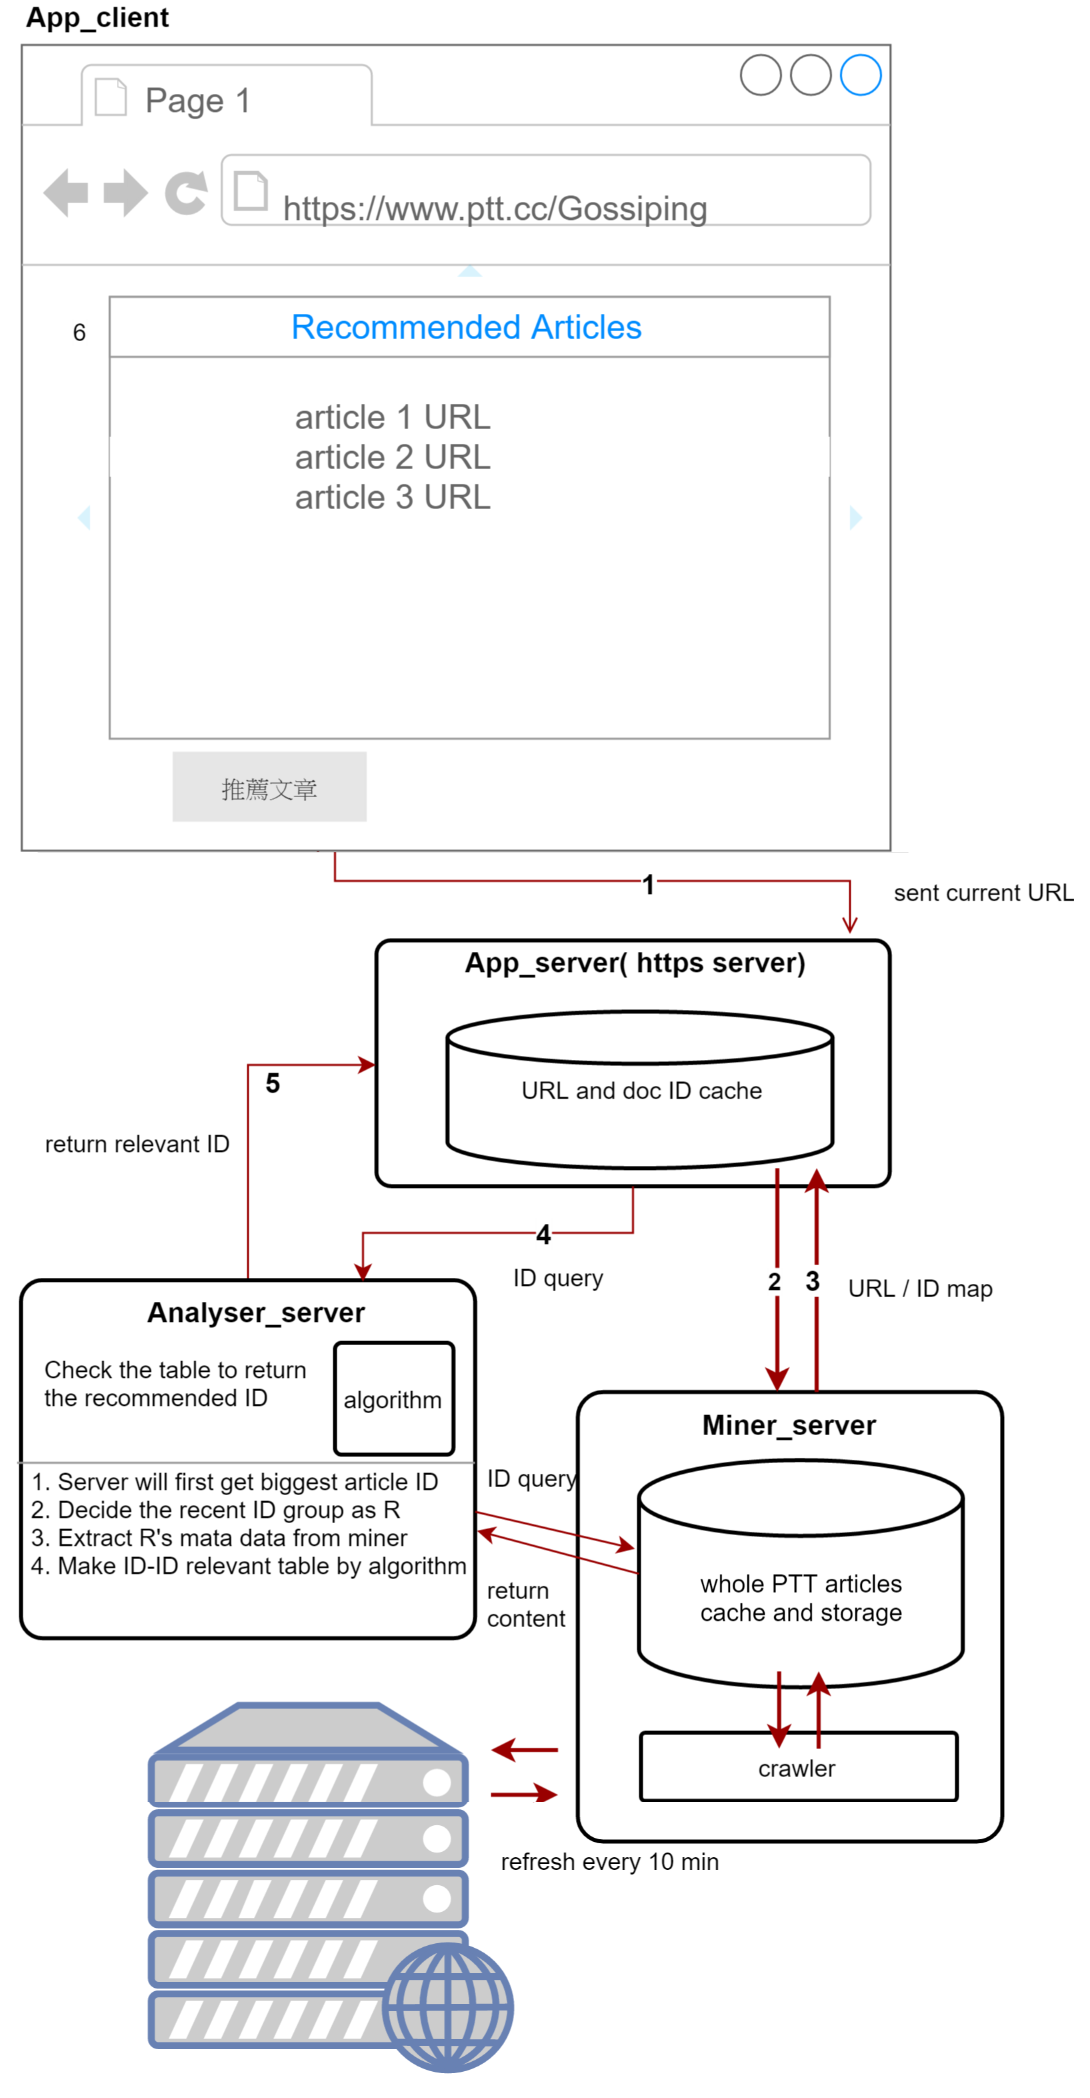
\includegraphics[scale=0.46]{structure.png}
\end{center}
In this report, we will first demonstrate how we design the recommender system in brief and then give the work flow of our recommender. Second, we will show details of how to find relevant articles that our system would recommend. Finally, we will show experiment of our system and give the distribution table of work.   


\subsection{\label{sec:level2}Component Design}
To recommend articles from articles on the web ptt, we have to first crawl all the articles from ptt to our Miner\_server. The Miner\_server will use L2 cache structure to store the data and update it periodically. The Miner will also give a special ID number based on articles' URL. We will have a Analyser\_server that will first read all articles from Miner based on ID and predict the relevant articles of each ID so as to make a table and keep it in the memory. After building the environments, our App\_server will serve as the bridge from users to our system. It will give recommended articles based on the URL that the user is reading now. The work flow of our system is given below and summarized as the graph on the left: 
\begin{enumerate}
\item[1] The App\_client will sent URL of this page and ask server to output the relevant articles when user opens a new article.
\item[2$\sim$3] Server asks Miner the corresponding ID of this URL and get return from Miner.
\item[4] Server asks Analyser to return the relevant articles' ID.   
\item[5] Analyser checks the pre-build table to answer the request and App\_server will also ask the corresponding URL of Analyser's return and finally return to the client.
\item[6] Client will make a pop-up window containing the hyper-links of recommended articles when user clicks the "推薦文章" bottom.
\end{enumerate}

\subsection{\label{sec:level3} Details of Retrieval}
In our analyser, we use some open source on github such as cppjieba \footnote{https://github.com/yanyiwu/cppjieba} and opencc \footnote{https://github.com/BYVoid/OpenCC} to help us divide both content and title of the article into chunks and then use BM25 model to calculate retrieval status value so as to predict the relevant articles, note that cppjieba is designed for simplified Chinese so we first use opencc to translate the articles so as to avoid some encoding bugs and increase precision, the procedure can be summarized as the graph below: 
\begin{center}
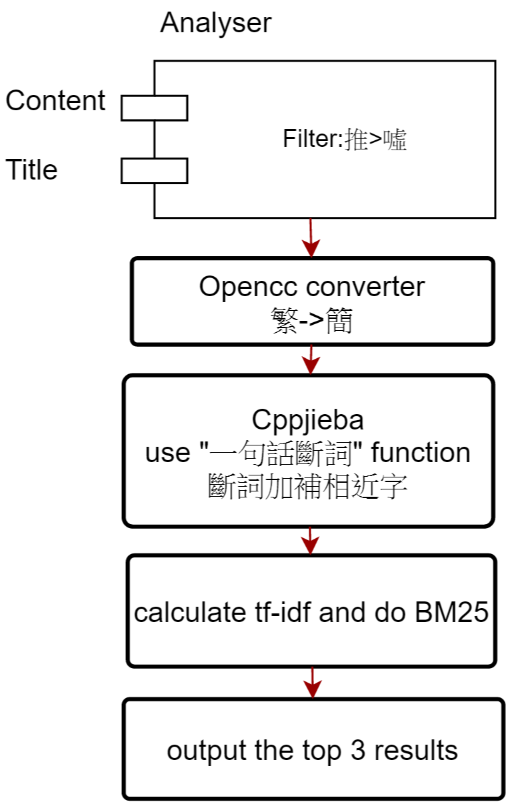
\includegraphics[scale=0.55]{retrieval.png}
\end{center}
In our BM25 model, we set $k_1$=1.5,b=0.75 and use the following formula:
\begin{footnotesize}
$$RSV_d=\sum_{t\in q}\log(\frac{N-df_t+0.5}{df_t+0.5})\cdot\frac{(k_1+1)tf_{t,d}}{k_1((1-b)+b*(L_d/L_{ave}))+tf_{t,d}}$$
\end{footnotesize}
\section{Experiment}
\begin{center}
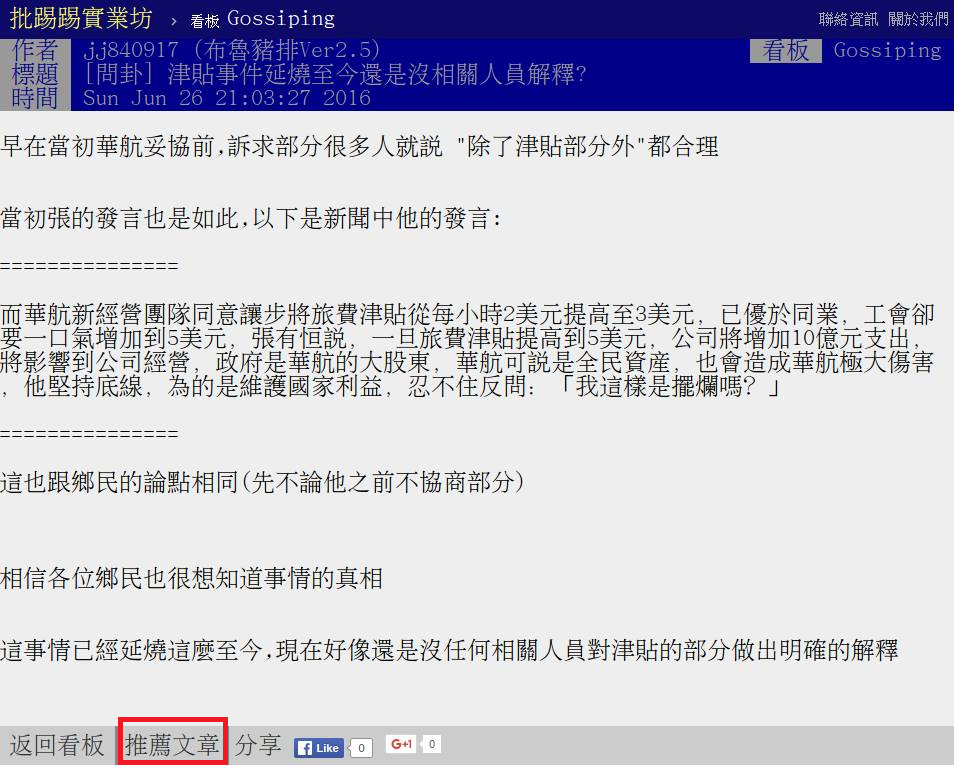
\includegraphics[scale=0.5]{experiment1.png}
\end{center}
\begin{center}
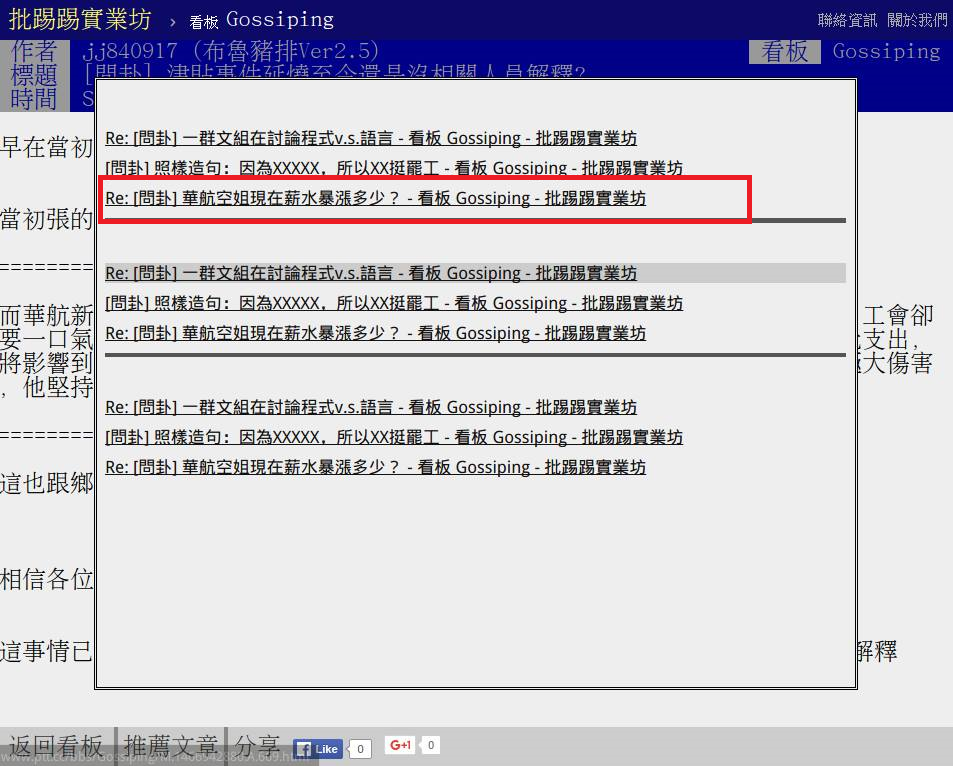
\includegraphics[scale=0.5]{experiment2.png}
\end{center}
\begin{center}
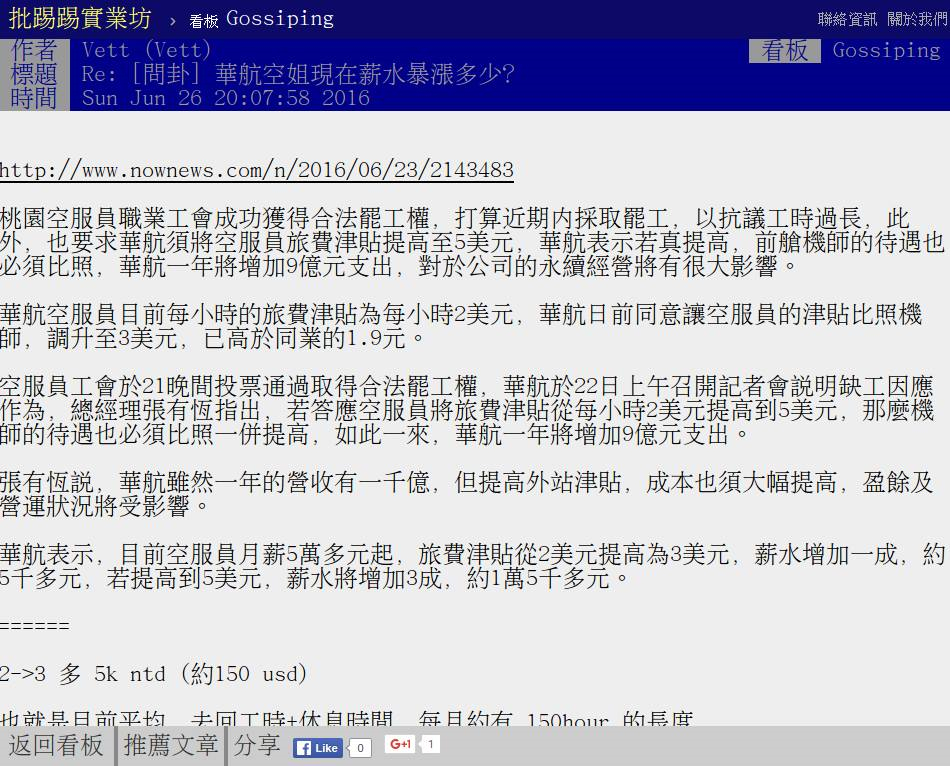
\includegraphics[scale=0.5]{experiment3.png}
\end{center}
\section{Distribution of work}
\begin{center}
\begin{tabular}{|l|l|}
\hline
ID        & work                        \\  \specialrule{2.5pt}{0pt}{0pt}
b01902013 & Analyser                    \\ \hline
b01902065 & Survey and report           \\ \hline
b01902109 & Code manager and everything \\ \hline
b01902103 & Miner                       \\ \hline
\end{tabular}
\end{center}
\section{Future work}
To be honest, we try to do sentiment analysis on web PTT at first. We follow the professor's advice and then survey Bing-Liu's paper\footnote{https://www.cs.uic.edu/$\sim$liub/publications/kdd04-revSummary.pdf} and tutorial\footnote{https://www.cs.uic.edu/$\sim$liub/FBS/Sentiment-Analysis-tutorial-AAAI-2011.pdf}. In this paper,professor Liu says that he will first divide the content of article into chunks(noun) and use the modifier of chunks (adjective) to be the opinion word. The major problem is how to learn the sentiment of each opinion words. Professor Liu will first label 30 adjectives as the seed and then iteratively search synonyms and antonyms of labelled word on WorldNet to expend the labelled opinion words. We try to mimic his work but find out that the Chinese Worldnet provided by LOPE Lab is somewhat broken and very hard to use so we narrow ourself to just recommend articles on web ptt without doing sentiment analysis. In the future, we wish we can know how to use the Chinese Worldnet to do sentiment analysis on PTT and we will try to publish our report to the chrome extension market.  

\end{document}
%
% ****** End of file aipsamp.tex ******


